Über die URL \url{https://nc.electribez.de/index.php/login} kommt ihr zur Verwaltungskonsole auf unserem Raspi-Nextcloud Server. \\
\ \\
Bitte beachtet, dass es sich um eine verschlüsselte ,,https://`` Verbindung über Port 443 handelt.\\

\begin{minipage}[t]{\textwidth}
  \centering
  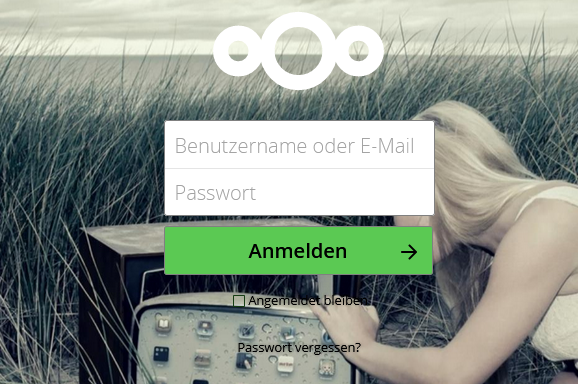
\includegraphics[height=5cm]{pictures/Nextcloudlogin.png}
  \captionof{figure}{Nextcloud Login}
  \label{img:Nextcloudlogin}
\end{minipage}

\subsection{Webinterface}
Zunächst solltet ihr euer Password ändern, welches ihr vom Admin zugewiesen bekommen habt. Falls ihr einen Script-Blocker verwendet fügt electribez.de als ausnahme hinzu.\\
Ihr könnt nun über das Webinterface auf die Dateien des Wak-Lab zugreifen.\\
 
\begin{minipage}[t]{\textwidth}
  \centering
  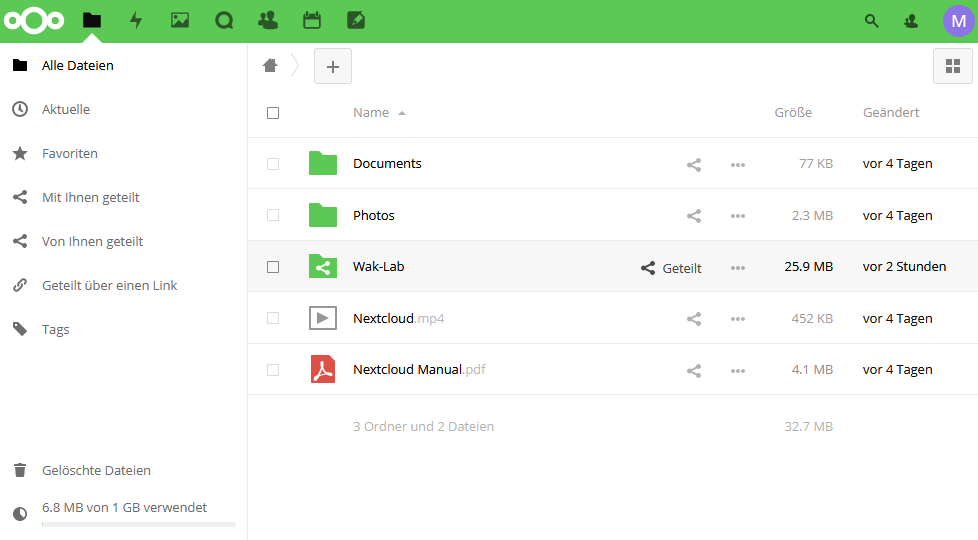
\includegraphics[height=6cm]{pictures/NextcloudWebinterface.png}
  \captionof{figure}{Nextcloud Web-Interface}
  \label{img:NextcloudWebinterface}
\end{minipage}


\subsubsection{Kalender}
\begin{minipage}[t]{\textwidth}
  \centering
  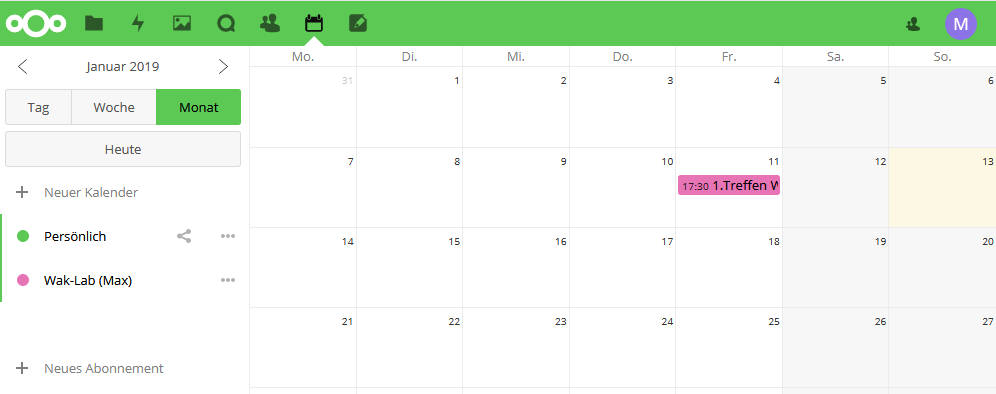
\includegraphics[height=6cm]{pictures/NextcloudKalender.png}
  \captionof{figure}{Nextcloud Kalender}
  \label{img:NextcloudKalender}
\end{minipage}


\subsection{Client Installieren}
Passende Clienten findet ihr auf \url{https://nextcloud.com/install/}\\
\ \\
Der Nexcloud Clienent stellt euch einen ständig aktualisierte Kopie des Servers in C:\textbackslash Users\textbackslash Username\textbackslash Nextcloud zur Verfügung. Dort können wir gemeinsam an Inhalten arbeiten. Vorsicht, wenn 2 Leute an einen Thema arbeiten.\\
 
\begin{minipage}[t]{\textwidth}
  \centering
  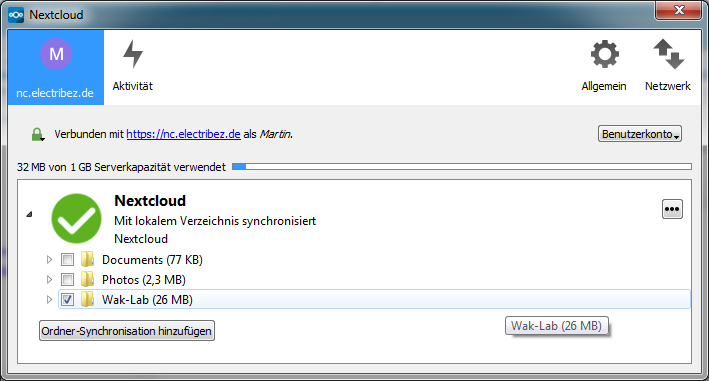
\includegraphics[height=5cm]{pictures/NextcloudWinClient.png}
  \captionof{figure}{Nextcloud Windows Client}
  \label{img:NextcloudWinClient}
\end{minipage}





